% The P2 moments of the tangent on TET10: the eleven quadrature points and four vertices, the ten
% stored moments M^ab (a <= b), and the moment schedule of the application (compress the increment
% to the vertex derivatives, sixteen block contractions, expand).
\documentclass[border=2pt]{standalone}
% Shared preamble of the format diagrams: colours of the paper's figures (paper_figures.py) and
% the drawing styles.  Each diagram is a standalone document built to a PDF of the text width.
\usepackage{amsmath,amssymb}
\usepackage{tikz}
\usetikzlibrary{arrows.meta,calc,decorations.pathreplacing,patterns,positioning}

\definecolor{cindex}{HTML}{BDBDBD}  % column indices, offsets, row pointers
\definecolor{cvalue}{HTML}{6E6E6E}  % floating-point values (BSR)
\definecolor{cpoint}{HTML}{1B9E77}  % quadrature-point store
\definecolor{celem}{HTML}{1F78B4}   % element matrix
\definecolor{cqbsr}{HTML}{A6761D}   % quantized BSR
\definecolor{cscale}{HTML}{E6AB02}  % scales
\definecolor{cmean}{HTML}{7570B3}   % f32 element mean

\tikzset{
  >={Stealth[length=4pt]},
  grid/.style={draw=black!45, line width=0.25pt},
  frame/.style={draw=black!70, line width=0.5pt},
  title/.style={font=\small\bfseries, anchor=west, inner sep=0pt},
  lab/.style={font=\footnotesize, inner sep=1pt},
  note/.style={font=\scriptsize, text=black!75, inner sep=1pt, execute at begin node={\hyphenpenalty=10000\exhyphenpenalty=10000}},
  num/.style={font=\tiny, inner sep=0pt},
  brace/.style={decorate, decoration={brace, amplitude=3pt, raise=1pt}, line width=0.4pt},
  arr/.style={->, line width=0.5pt, black!70},
  pad/.style={pattern=north east lines, pattern color=black!30},
}

% \cell{x}{y}{w}{h}{fill}: a filled rectangle with a thin outline, lower-left corner at (x,y).
\newcommand{\cell}[5]{\filldraw[fill=#5, grid] (#1,#2) rectangle ++(#3,#4);}
% \blk{x}{y}{s}{fill}: a 3x3 block of side s with its 3x3 entry grid.
\newcommand{\blk}[4]{%
  \filldraw[fill=#4, grid] (#1,#2) rectangle ++(#3,#3);
  \draw[draw=white, line width=0.25pt] (#1,#2) ++(#3/3,0) -- ++(0,#3) ++(#3/3,0) -- ++(0,-#3);
  \draw[draw=white, line width=0.25pt] (#1,#2) ++(0,#3/3) -- ++(#3,0) ++(0,#3/3) -- ++(-#3,0);
  \draw[grid] (#1,#2) rectangle ++(#3,#3);}
% \vthree{x}{y}{fill}: a 3-vector (one node's components) as three small cells, left end at (x,y).
\newcommand{\vthree}[3]{\foreach \k in {0,1,2} \filldraw[fill=#3, grid] (#1+\k*0.14,#2) rectangle ++(0.14,0.14);}
% \op{x}{y}{symbol}: an operation in a small circle.
\newcommand{\op}[3]{\node[circle, draw=black!70, line width=0.4pt, inner sep=0.5pt, minimum size=9pt, font=\tiny] at (#1,#2) {#3};}

\begin{document}
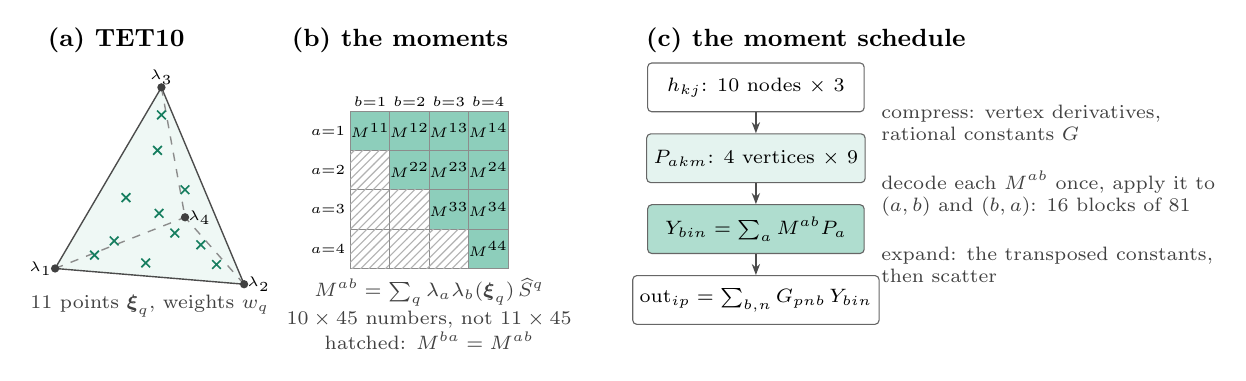
\begin{tikzpicture}
  \tikzset{
    box/.style={draw=black!60, line width=0.4pt, rounded corners=1.5pt, font=\scriptsize, align=center,
                inner sep=2.5pt, minimum height=0.62cm, minimum width=2.75cm},
  }
  % ---------------------------------------------------------------- (a) points and vertices
  \node[title] at (0, 3.45) {(a) TET10};
  \coordinate (v1) at (0.1,0.55); \coordinate (v2) at (2.5,0.35); \coordinate (v3) at (1.45,2.85);
  \coordinate (v4) at (1.75,1.2);
  \filldraw[fill=cpoint!7, draw=none] (v1) -- (v2) -- (v3) -- cycle;
  \draw[frame] (v1) -- (v2) -- (v3) -- cycle;
  \draw[frame, dashed, draw=black!45] (v1) -- (v4) (v2) -- (v4) (v3) -- (v4);
  \foreach \v/\pos [count=\a] in {v1/left, v2/right, v3/above, v4/right} {
    \fill[black!75] (\v) circle (1.5pt);
    \node[num, \pos=1pt] at (\v) {$\lambda_{\a}$};
  }
  \foreach \x/\y in {1.42/1.25, 0.85/0.9, 1.95/0.85, 1.4/2.05, 1.25/0.62, 1.75/1.55, 1.0/1.45,
                     0.6/0.72, 2.15/0.6, 1.45/2.5, 1.62/1.0}
    \draw[cpoint!80!black, line width=0.6pt] (\x-0.055,\y-0.055) -- (\x+0.055,\y+0.055) (\x-0.055,\y+0.055) -- (\x+0.055,\y-0.055);
  \node[note, anchor=north, align=center] at (1.3, 0.25) {$11$ points $\boldsymbol{\xi}_q$, weights $w_q$};

  % ---------------------------------------------------------------- (b) the ten moments
  \begin{scope}[shift={(3.85,0.55)}]
    \node[title] at (-0.75, 2.9) {(b) the moments};
    \def\s{0.5}
    \foreach \a in {1,...,4} \foreach \b in {1,...,4} {
      \pgfmathsetmacro{\x}{(\b-1)*\s}\pgfmathsetmacro{\y}{(4-\a)*\s}
      \ifnum\a>\b
        \filldraw[fill=white, grid] (\x,\y) rectangle ++(\s,\s); \fill[pad] (\x,\y) rectangle ++(\s,\s);
      \else
        \filldraw[fill=cpoint!50, grid] (\x,\y) rectangle ++(\s,\s);
        \node[num] at (\x+\s/2, \y+\s/2) {$M^{\a\b}$};
      \fi
    }
    \foreach \a in {1,...,4} {
      \node[num, anchor=east] at (-0.06, {(4-\a)*\s+\s/2}) {$a{=}\a$};
      \node[num, anchor=south] at ({(\a-1)*\s+\s/2}, 4*\s+0.05) {$b{=}\a$};
    }
    \node[note, anchor=north, align=center] at (1.0, -0.08)
      {$M^{ab} = \sum_q \lambda_a\lambda_b(\boldsymbol{\xi}_q)\, \widehat S^{q}$\\[1pt] $10\times45$ numbers, not $11\times45$\\[1pt] hatched: $M^{ba}=M^{ab}$};
  \end{scope}

  % ---------------------------------------------------------------- (c) the moment schedule
  \begin{scope}[shift={(7.6,0)}]
    \node[title] at (0, 3.45) {(c) the moment schedule};
    \node[box, fill=white] (h) at (1.4, 2.85) {$h_{kj}$: $10$ nodes $\times$ $3$};
    \node[box, fill=cpoint!12] (p) at (1.4, 1.95) {$P_{akm}$: $4$ vertices $\times$ $9$};
    \node[box, fill=cpoint!35] (y) at (1.4, 1.05) {$Y_{bin} = \sum_{a} M^{ab} P_{a}$};
    \node[box, fill=white] (o) at (1.4, 0.15) {$\mathrm{out}_{ip} = \sum_{b,n} G_{pnb}\, Y_{bin}$};
    \draw[arr] (h) -- (p); \draw[arr] (p) -- (y); \draw[arr] (y) -- (o);
    \node[note, anchor=west, align=left] at (2.95, 2.4) {compress: vertex derivatives,\\rational constants $G$};
    \node[note, anchor=west, align=left] at (2.95, 1.5) {decode each $M^{ab}$ once, apply it to\\$(a,b)$ and $(b,a)$: $16$ blocks of $81$};
    \node[note, anchor=west, align=left] at (2.95, 0.6) {expand: the transposed constants,\\then scatter};
  \end{scope}
\end{tikzpicture}
\end{document}
